%%%%%%%%%%%%%%%%%%%%%%%%%%%%%%%%%%%%%%%%%%%%%%%%%%%%%%%%%%
%   Autoren des verwendeten Templates:
%   Prof. Dr. Bernhard Drabant
%   Prof. Dr. Dennis Pfisterer
%   Prof. Dr. Julian Reichwald
%%%%%%%%%%%%%%%%%%%%%%%%%%%%%%%%%%%%%%%%%%%%%%%%%%%%%%%%%%

\documentclass[fontsize=12pt,BCOR=5mm,DIV=12,parskip=half,listof=totoc,
               paper=a4,toc=bibliography,pointlessnumbers]{scrreprt}

               %toc=listof,listof=entryprefix,

\makeindex

%% Elementare Pakete, Konfigurationen und Definitionen werden geladen (gegebenenfalls anpassen)
% !TEX root =  master.tex

%%%%%%%%%%%%%%%%%%%%%%%%%%%%%%%%%%%%%%%%%%%%%%%%%%%%%%%%%%%%%%%%%%
%	ANLEITUNG:
% Passen Sie gegebenenfalls alle Stellen im Dokument an, die mit
% @stud
% markiert sind.
%%%%%%%%%%%%%%%%%%%%%%%%%%%%%%%%%%%%%%%%%%%%%%%%%%%%%%%%%%%%%%%%%%

%%
%% @stud
%%
%% LANGUAGE SETTINGS
\usepackage[ngerman]{babel}				% german language
\usepackage[german=quotes]{csquotes}	% correct quoting using \enquote{}
%\usepackage[english]{babel}			% english language
% \usepackage{csquotes}					% correct quoting using \enquote{}

\usepackage{makeidx}					% allows index generation
\usepackage{listings}					% Format Listings properly
\usepackage{lipsum}						% Blindtext
\usepackage{graphicx}					% use various graphics formats
\usepackage[german]{varioref}			% nicer references \vref
\usepackage[format=plain]{caption}		% better Captions (format=plain to avoid hanging indentation)
\usepackage{booktabs}					% nicer Tabs
\usepackage[hidelinks=true]{hyperref}	% keine roten Markierungen bei Links
\usepackage{fnpct}						% Correct superscripts
\usepackage{calc}						% Used for extra space below footsepline, in particular
\usepackage{array}						% Better Array & Tabular environments
\usepackage{acronym}					% Allows using acronyms
\usepackage{algorithm}					% provides block command \algorithm
\usepackage{algpseudocode}				% Typesetting pseudocode
\usepackage{setspace}					% Allows setting line-spacing
\usepackage{tocloft}					% better table of contents, lists of figures/tables
\usepackage{tikz}						% Used for drawing directly in LaTeX

%% Schriftarten- und Zeichenpakete
\usepackage[T1]{fontenc}				% For font encodings
\usepackage[utf8]{inputenc}				% For input encodings

%%
%% @stud
%%
%%	FONT SELECTION: Schriftarten und Schriftfamilie
%%%%%%%%%%%%%
%% SCHRIFTART
%%%%%%%%%%%%%
% 0) without decomment: normal font families
% ...
% 1) Latin Modern
%\usepackage{lmodern}
% 2) Times
%\usepackage{mathptmx}
% 3) Helvetica
%\usepackage[scaled=.92]{helvet}
%%%%%%%%%%%%%%%%%%
%%	SCHRIFTFAMILIE
%%%%%%%%%%%%%%%%%%
% ohne Serifen
\renewcommand*{\familydefault}{\sfdefault}
\addtokomafont{disposition}{\sffamily}
%
% mit Serifen
%\renewcommand*{\familydefault}{\rmdefault}
%\addtokomafont{disposition}{\rmfamily}
%
% Typewriter
%\renewcommand*{\familydefault}{\ttdefault}
%\addtokomafont{disposition}{\ttfamily}

%%
%% @stud
%%
%% Uncomment the following lines to support hard URL breaks in bibliography
%\apptocmd{\UrlBreaks}{\do\f\do\m}{}{}
%\setcounter{biburllcpenalty}{9000}% Kleinbuchstaben
%\setcounter{biburlucpenalty}{9000}% Großbuchstaben

%%
%% @stud
%%
%% FOOTNOTES: Count footnotes over chapters
%% \counterwithout{footnote}{chapter}

%	ACRONYMS
\makeatletter
\@ifpackagelater{acronym}{2015/03/20}
{\renewcommand*{\aclabelfont}[1]{\textbf{{\acsfont{#1}}}}}{}
\makeatother

%	LISTINGS
% @stud: ggf. Namen/Text anpassen (englisch)
\renewcommand{\lstlistingname}{Quelltext}
\renewcommand{\lstlistlistingname}{Quelltextverzeichnis}
\lstset{numbers=left,
	numberstyle=\tiny,
	captionpos=b,
	basicstyle=\ttfamily\small}

%	ALGORITHMS
% @stud: ggf. Namen/Text anpassen (englisch)
\renewcommand{\listalgorithmname}{Algorithmenverzeichnis}
\floatname{algorithm}{Algorithmus}

%	PAGE HEADER / FOOTER
%	Warning: There are some redefinitions throughout the master.tex-file!  DON'T CHANGE THESE REDEFINITIONS!
\RequirePackage[automark]{scrlayer-scrpage}
%alternatively with separation lines: \RequirePackage[automark,headsepline,footsepline]{scrlayer-scrpage}

\renewcommand{\chaptermarkformat}{}
\RedeclareSectionCommand[beforeskip=0pt]{chapter}
\clearpairofpagestyles

%\ifoot[\rule{0pt}{\ht\strutbox+\dp\strutbox}DHBW Mannheim]{\rule{0pt}{\ht\strutbox+\dp\strutbox}DHBW Mannheim}
\ofoot[\rule{0pt}{\ht\strutbox+\dp\strutbox}\pagemark]{\rule{0pt}{\ht\strutbox+\dp\strutbox}\pagemark}
\ohead{\headmark}

\newcommand{\TitelDerArbeit}[1]{\def\DerTitelDerArbeit{#1}\hypersetup{pdftitle={#1}}}
\newcommand{\AutorDerArbeit}[1]{\def\DerAutorDerArbeit{#1}\hypersetup{pdfauthor={#1}}}
\newcommand{\Kurs}[1]{\def\DieKursbezeichnung{#1}}
\newcommand{\Studiengangsleiter}[1]{\def\DerStudiengangsleiter{#1}}
\newcommand{\WissBetreuer}[1]{\def\DerWissBetreuer{#1}}
\newcommand{\Bearbeitungszeitraum}[1]{\def\DerBearbeitungszeitraum{#1}}
\newcommand{\Abgabedatum}[1]{\def\DasAbgabedatum{#1}}
\newcommand{\Matrikelnummer}[1]{\def\DieMatrikelnummer{#1}}
\newcommand{\Studienrichtung}[1]{\def\DieStudienrichtung{#1}}
\newcommand{\ArtDerArbeit}[1]{\def\DieArtDerArbeit{#1}}
\newcommand{\Literaturverzeichnis}{Literaturverzeichnis}

\newcommand{\settingBibFootnoteCite}{
	\setlength{\bibparsep}{\parskip}		  % Add some space between biblatex entries in the bibliography
	\addbibresource{bibliography.bib}	    % Add file bibliography.bib as biblatex resource
	\DefineBibliographyStrings{ngerman}{andothers = {{et\,al\adddot}},}
}

\newcommand{\setTitlepage}{
	% !TEX root =  master.tex
% @stud: ggf. Namen/Text anpassen (englisch)
\begin{titlepage}
\begin{minipage}{\textwidth}
		\vspace{-2cm}
		\noindent \hfill 
\includegraphics{\imagedir/logo.jpg}
\end{minipage}
\vspace{1em}
%\sffamily
\begin{center}
	{\textsf{\large Duale Hochschule Baden-W\"urttemberg Mannheim}}\\[4em]
	{\textsf{\textbf{\large{\DieArtDerArbeit}arbeit}}}\\[6mm]
	{\textsf{\textbf{\Large{}\DerTitelDerArbeit}}} \\[1.5cm]
	{\textsf{\textbf{\large{}Studiengang Informatik}}\\[6mm]
	\textsf{\textbf{Studienrichtung \DieStudienrichtung}}}\vspace{10em}

	\begin{minipage}{\textwidth}
		\begin{tabbing}
		Wissenschaftliche(r) Betreuer(in): \hspace{0.85cm}\=\kill
		Verfasser:innen: \> \AutorinnenDerArbeit \\[1.5mm]
		Matrikelnummern: \> \DieMatrikelnummer \\[1.5mm]
		Kurs: \> \DieKursbezeichnung \\[1.5mm]
		Studiengangsleiter: \> \DerStudiengangsleiter \\[1.5mm]
		Wissenschaftliche(r) Betreuer(in): \> \DerWissBetreuer \\[1.5mm]
		Bearbeitungszeitraum: \> \DerBearbeitungszeitraum\\[1.5mm]
%		alternativ:\\[1.5mm]
%		Eingereicht: \> \DasAbgabedatum
		\end{tabbing}
	\end{minipage}
\end{center}
\end{titlepage}
	\pagenumbering{roman} % Römische Seitennummerierung
	\normalfont
}

\newcommand{\initializeText}{
	\clearpage
	\ihead{\chaptername~\thechapter} % Neue Header-Definition
	\pagenumbering{arabic}           % Arabische Seitenzahlen
}

\newcommand{\initializeBibliography}{
	\ihead{}
	\printbibliography[title=\Literaturverzeichnis]
	\cleardoublepage
}

\newcommand{\initializeAppendix}{
	\appendix
  \ihead{}
  \cftaddtitleline{toc}{chapter}{Anhang}{}
}



%%
%% @stud
%%
%% PERSÖNLICHE ANGABEN (BITTE VOLLSTÄNDIG EINGEBEN zwischen den Klammern: {...})
%%
\ArtDerArbeit{Studien}
\TitelDerArbeit{<Titel Ihrer Arbeit>}
\AutorDerArbeit{Jakob Kautz, Olivier Stenzel, Val Richter}
\Kurs{TINF21AI1}
\Studienrichtung{Angewandte Informatik}
\Matrikelnummer{<Martikelnummern>}
\Studiengangsleiter{Prof. Dr. Holger D. Hofmann}
\WissBetreuer{Prof. Dr. Eckhardt Kruse}
\Bearbeitungszeitraum{01.10.2023 -- 16.04.2024}
\Abgabedatum{dd.mm.yyyy}

%%
%% @stud
%%
%% BIBLIOGRAPHY (@stud: Bibliographie-Stil wählen - Position und Indizierung)
%%  Auswahl zwischen:
%%   NUMERIC Style
%%   IEEE Style
%%   ALPHABETIC Style
%%   HARVARD Style
%%   CHICAGO Style
%%   (oder eigenen zulässigen Stil wählen)
%%
%%%%%%%%%%%%%
%% Zitierstil
%%%%%%%%%%%%%
% NUMERIC Style - e. g. [12]
%\newcommand{\indextype}{numeric}
%
% IEEE Style - numeric kind of style
%\newcommand{\indextype}{ieee}
%
% ALPHABETIC Style - e. g. [AB12]
\newcommand{\indextype}{alphabetic}
%
% HARVARD Style
%\newcommand{\indextype}{apa}
%
% CHICAGO Style
%\newcommand{\indextype}{authoryear}
%
%%%%%%%%%%%%%%%%%%%%%%
%% Position des Zitats
%%%%%%%%%%%%%%%%%%%%%%
\newcommand{\position}{inline}
%
% (!!) FOOTNOTE POSITION NOT RECOMMENDED IN MINT DOMAIN:
%\newcommand{\position}{footnote}

%% Final: Setzen des Zitierstils und der Zitatposition
\usepackage[backend=biber, autocite=\position, style=\indextype]{biblatex}
\usepackage{enumerate}
\usepackage{cleveref}
\settingBibFootnoteCite

%%
%% Definitionen und Commands
%%
\newcommand{\abs}{\par\vskip 0.2cm\goodbreak\noindent}
\newcommand{\nl}{\par\noindent}
\newcommand{\mcl}[1]{\mathcal{#1}}
\newcommand{\nowrite}[1]{}
\newcommand{\NN}{{\mathbb N}}
\newcommand{\imagedir}{img}
\DeclareRobustCommand{\micro}{\mu}

\makeindex

\begin{document}

\setTitlepage
\addcontentsline{toc}{chapter}{Titelseite}

%%%%%%%%%%%%%%%%%%%%%%%%%%%%%%%%%%%
% EHRENWÖRTLICHE ERKLÄRUNG
%
% @stud: ewerkl.tex bearbeiten
%
% !TEX root =  master.tex
\clearpage
\chapter*{Ehrenwörtliche Erklärung}

% Wird die folgende Zeile auskommentiert, erscheint die ehrenwörtliche
% Erklärung im Inhaltsverzeichnis.

% \addcontentsline{toc}{chapter}{Ehrenwörtliche Erklärung}
Wir versicheren hiermit, dass wir die vorliegende Arbeit mit dem Titel ``\textit{\DerTitelDerArbeit}'' selbstständig verfasst und
keine anderen als die angegebenen Quellen und Hilfsmittel benutzt haben. Wir versicheren zudem, dass die eingereichte elektronische Fassung mit der gedruckten Fassung übereinstimmt.

\vspace{3cm}
Ort, Datum \hfill \AutorinnenDerArbeit

\addcontentsline{toc}{chapter}{Ehrenwörtliche Erklärung}
\cleardoublepage
%%%%%%%%%%%%%%%%%%%%%%%%%%%%%%%%%%%

%%%%%%%%%%%%%%%%%%%%%%%%%%%%%%%%%%%
% VERZEICHNISSE und ABSTRACT
%
% @stud: ggf. nicht benötigte Verzeichnisse auskommentieren/löschen
%
\tableofcontents
\addcontentsline{toc}{chapter}{Inhaltsverzeichnis}
\cleardoublepage

% Abbildungsverzeichnis
\phantomsection
\addcontentsline{toc}{chapter}{\listfigurename}
\listoffigures
\cleardoublepage

%	Tabellenverzeichnis
\phantomsection
\addcontentsline{toc}{chapter}{\listtablename}
\listoftables
\cleardoublepage

%	Listingsverzeichnis / Quelltextverzeichnis
\lstlistoflistings
\cleardoublepage

% Algorithmenverzeichnis
\listofalgorithms
\cleardoublepage

% Abkürzungsverzeichnis
% @stud: abkürzungen.tex bearbeiten
\input{abkürzungen}
\cleardoublepage

% 1,5 Zeilenabstand schon ab dem Abstrakt
\onehalfspacing

%	Kurzfassung / Abstract
% @stud: abstract.tex bearbeiten
%%%%%%%%%%%%%%%%%%%%%%%%%%%%%%%%%%%%%%%%%%%%%%%%%%%%%%%%%%
%   Autoren des Abschnitts:
%   ???
%%%%%%%%%%%%%%%%%%%%%%%%%%%%%%%%%%%%%%%%%%%%%%%%%%%%%%%%%%

% !TEX root =  master.tex
\chapter*{Kurzfassung (Abstract)}
\addcontentsline{toc}{chapter}{Kurzfassung (Abstract)}

\paragraph*{Deutsch:}

Hier können Sie die Kurzfassung (engl.~Abstract) der Arbeit schreiben. Beachten Sie dabei die Hinweise zum Verfassen der Kurzfassung.

\paragraph*{Englisch:}

The same abstract in english.

\cleardoublepage

%%%%%%%%%%%%%%%%%%%%%%%%%%%%%%%%%%%%%%%%%%%%%%%%%%%%%%%%%%%%%%%%%%%%%%%%%%%%%%%%%%%%%%%%%%
% KAPITEL UND ANHÄNGE
%
% @stud:
%   - nicht benötigte: auskommentieren/löschen
%   - neue: bei Bedarf hinzufügen mittels input-Kommando an entsprechender Stelle einfügen
%%%%%%%%%%%%%%%%%%%%%%%%%%%%%%%%%%%%%%%%%%%%%%%%%%%%%%%%%%%%%%%%%%%%%%%%%%%%%%%%%%%%%%%%%%

\initializeText

%%%%%%%%%%%%%%%%%%%%%%%%%%%%%%%%%%%
% KAPITEL
%
% @stud: einzelne Kapitel bearbeiten und eigene Kapitel hier einfügen
%%%%%%%%%%%%%%%%%%%%%%%%%%%%%%%%%%%%%%%%%%%%%%%%%%%%%%%%%%
%   Autoren des Abschnitts:
%   Olivier Stenzel
%%%%%%%%%%%%%%%%%%%%%%%%%%%%%%%%%%%%%%%%%%%%%%%%%%%%%%%%%%

% !TEX root =  master.tex
\chapter{Einleitung} \label{einleitung}
\chapterauthor{Olivier Stenzel}

\nocite{*}

Im Rahmen dieser Studienarbeit wird ein selbstspielendes Klavier konzipiert und gebaut.
Klaviermusik findet in zahlreichen Umgebungen ihren Einsatz: von der Untermalung in Hotel-Lobbys durch Bar-Pianist:innen bis hin zu privaten Haushalten,
wo sie zur Atmosphäre und Unterhaltung beiträgt.
Vor diesem Hintergrund könnte ein selbstspielendes Klavier, speziell in Bereichen, wo traditionellerweise Live-Musiker:innen engagiert werden,
einen signifikanten Mehrwert darstellen.

Obwohl die Technologie der selbstspielenden Klaviere bereits etabliert ist, bleiben die Kosten für solche Instrumente mit Preisen,
die leicht 10.000 Euro überschreiten können, eine beträchtliche Hürde \cite*{YamahaU1}.
Diese finanzielle Barriere limitiert den Zugang zu dieser Technologie für eine breite Nutzerbasis erheblich.
Angesichts dieser Preisgestaltung ist eine wesentliche Motivation dieser Arbeit die Entwicklung einer deutlich preisgünsigeren Alternative.
Das Ziel ist es, ein Instrument zu konzipieren, das die wesentlichen Funktionalitäten seines professionellen Pendants beibehält,
jedoch zu einem Bruchteil der Kosten realisiert werden kann.
Durch dieses Vorhaben sollen selbstspielende Klaviere einem breiteren Publikum zugänglich gemacht werden.




%%%%%%%%%%%%%%%%%%%%%%%%%%%%%%%%%%%%%%%%%%%%%%%%%%%%%%%%%%
%   Autoren des Abschnitts:
%   Olivier Stenzel
%%%%%%%%%%%%%%%%%%%%%%%%%%%%%%%%%%%%%%%%%%%%%%%%%%%%%%%%%%
% !TEX root =  master.tex
\chapter{Ziele und Anforderungen} \label{Zielstellung}
\chapterauthor{Olivier Stenzel}

\nocite{*}


Das Kernanliegen dieser Arbeit ist die Entwicklung eines multifunktionalen Klaviers,
das sowohl manuell von Musiker:innen als auch automatisiert durch einen Computer bespielt werden kann.

Da es wünschenswert ist, dass Nutzer:innen auf eine breite Palette fertiger Stücke zugreifen und diese selbstständig erweitern können,
wäre eine Steuerung über den PC sinnvoll.
Neben der Auswahl von Musikstücken soll die Anwendung außerdem die Möglichkeit bieten,
die Wiedergabegeschwindigkeit und die Lautstärke individuell anzupassen.

In Anlehnung an die Funktionsweise populärer Musikplayer wird angestrebt,
dass die Wiedergabe nicht nur pausiert, sondern auch innerhalb eines Stücks frei navigiert werden kann.

% @Note(Val): Finde den erzwungenen Seitenumbruch hier eher unschön - gibt es einen Grund den zu haben?
\newpage

\section{Anforderungen} \label{sec:zielstellung-anforderungen}

% @Note(Val): Die Anforderungen werden nicht motiviert, sondern einfach gestellt.
% @Note(Val): Für die Desktop-Anwendung habe ich einiges an Motivation für die Anforderungen geschrieben
% Das ist gerade im Unterkapitel konzeptionSW-UI, aber sollte vielleicht hierher verschoben werden
% Eine ähnliche Motivation könnte für die restlichen Anforderungen auch geschrieben werden
Im Folgenden befinden sich die allgemeinen Anforderungen, die an dieses Projekt gestellt wurden,
um die Arbeit in kleinere Arbeitspakete aufteilen zu können.

% @Note(Kruse): Ggf. erklären was die Priorisierungen hier für uns und unsere Ergebnisse bedeutet

% @TODO(Val): Hinzufügen von
\begin{table}[ht]
    \centering
    \begin{tabular}{ | m{1cm} | m{2cm} | m{8cm} | m{2cm} | }
        \hline
        \textbf{Nr.} & \textbf{Kategorie} & \textbf{Anforderung} & \textbf{Priorität} \\
        \hline
        1 & \multirow{3}{2cm}{Allgemein} & Flexibilität: Das Klavier muss sowohl manuell als auch automatisch bespielbar sein. & Hoch \\
        \cline{1-1} \cline{3-4}
        2 & & Benutzerinterface: Entwicklung eines intuitiven Interfaces. & Hoch \\
        \cline{1-1} \cline{3-4}
        3 & & Budget: Gesamtkosten < 2000€. & Mittel \\
        \cline{1-1} \cline{3-4}
        4 & & Responsivität: Die Anwendung muss auf verschiedenen Computern mit Windows 10 und 11 laufen. & Mittel \\
        \cline{1-1} \cline{3-4}
        5 & & Performanz: Die Performanz soll mindestens die von professionellen Pianist:innen erreichen. & Mittel \\
        \cline{1-1} \cline{3-4}% @TODO(Jay): Muss in Fazit rein und besser definiert werden
        6 & & Spielbarkeit: Der Aufbau sollte dazu in der Lage sein, mindestens 10 Tasten gleichzeitig anspielen zu können & Mittel \\
        \hline
        7 & \multirow{2}{2cm}{Hardware} & Tastenbetätigung: Hardware muss in der Lage sein, Klaviertasten autonom zu bedienen. & Hoch \\
        \cline{1-1} \cline{3-4}
        8 & & Anpassbarkeit: Hardware-Komponenten müssen auf unterschiedliche Klaviertypen anpassbar sein. & Mittel \\
        \hline
        9 & \multirow{4}{2cm}{Software} & Musikstück-Auswahl: Nutzer:innen wählen Musikstücke über eine Desktop-Anwendung. & Hoch \\
        \cline{1-1} \cline{3-4}
        10 & & Wiedergabe-Kontrolle: Anpassung der Wiedergabegeschwindigkeit und Lautstärke. & Mittel \\
        \cline{1-1} \cline{3-4}
        11 & & Navigation: Möglichkeit, die Wiedergabe zu pausieren und innerhalb des Stücks zu navigieren. & Mittel \\
        \cline{1-1} \cline{3-4}
        12 & & MIDI-Integration: System muss MIDI-Dateien für die Erweiterung des Katalogs unterstützen. & Mittel \\
        \hline
    \end{tabular}
    \caption{Anforderungen an das selbstspielende Klavier}
    \label{table:anforderungen}
\end{table}



\section{Vorgehensweise} \label{sec:zielstellung-vorgehen}

In diesem Kapitel wird der geplante Ablauf des Projektes zur Entwicklung eines selbstspielenden Klaviers vorgestellt.
Die Vorgehensweise ist in mehrere Phasen unterteilt, die das parallele Arbeiten vereinfachen. % @Note(Val): Mehrere Phasen vereinfachen nicht das parallele Arbeiten, weil Phasen per Def. nacheinander ablaufen. Wenn dann können wir sagen, dass es in mehrere Teile geteilt wurde. Alternativ können wir auch einfach konkret sagen, dass wir es zwischen Software und Hardware geteilt haben

\subsubsection{Konzeptualisierung und Planung}\label{Vorgehensweise - Konzeptualisierung und Planung}
% @Note(Val): Soll das hier nur die Konzeptualisierung der Hardware sein?
% Dann wäre Hardware-Konzeptualisierung oder so besser als Name
% Dann lässt es sich aber auch mit Hardware-Implementierung zu "Hardware-Entwicklung" zusammen tun
% Dann wäre es zumindest symmetrisch zu Abschnitt "Software-Entwicklung"

Zu Beginn des Projektes stand die Konzeptualisierung, in der die grundlegenden Anforderungen an das System festgelegt wurden.
Besondere Aufmerksamkeit galt dabei der Schnittstelle zwischen der Hardware, die durch einen kompakten \ac{MC} gesteuert wird, und der Software der Desktop-Anwendung.
Die Planungsphase umfasst: % @Note(Val): Das ist nicht alles die Planungsphase though...

\begin{itemize}
    \item Definition der funktionalen Anforderungen an das Klavier. (siehe Kapitel \ref{sec:zielstellung-anforderungen})
    \item Auswahl der Ansteuerung-Hardware. (siehe Kapitel \ref{konzeptionHW})
    \item Bau der Ansteuerungs-Hardware. (siehe Kapitel \ref{umsetzungHW})
    \item Entwurf des Konzepts für die Desktop-Anwendung. (siehe Kapitel \ref{vorgehenSW})
    \item Entwicklung der Software. (siehe Kapitel \ref{umsetzungSW})
    \item Testen der Kombination aus Hard-und Software. (siehe Kapitel \ref{tests})
    \item Fazit. (siehe Kapitel \ref{fazit})
\end{itemize}

\subsubsection{Hardware-Implementierung}\label{Vorgehensweise - Hardware-Implementierung}

Nach der Konzeptualisierung folgte die Implementierungsphase der Hardware:

\begin{itemize}
    \item Auswahl und Testung von Komponenten, die in der Lage sind, die Klaviertasten autonom zu betätigen.
    \item Entwicklung eines Prototyps zur Überprüfung der Ansteuerung und Funktionalität der Tasten.
    \item Integration des \ac{MC}s in das Gesamtsystem und Programmierung der Steuerungslogik. % @Note(Val): Ist eigentlich Teil der Software, oder?
\end{itemize}

\subsubsection{Software-Entwicklung}\label{Vorgehensweise - Software-Entwicklung}

Parallel zur Hardware-Entwicklung wird die Software konzipiert und programmiert:

\begin{itemize}
    \item Entwicklung eines Kommunikationsprotokolls zwischen Anwendungsprogramm und \ac{MC}.
    \item Gestaltung der Benutzeroberfläche der Desktop-Anwendung, welche die Auswahl und Wiedergabe der Musikstücke ermöglicht.
    \item Implementierung von Funktionen zur Anpassung der Wiedergabegeschwindigkeit und Lautstärke.
    \item Entwicklung eines Systems zur Verwaltung und Erweiterung des Musik-Katalogs, einschließlich der Integration und des Parsings von MIDI-Dateien.
\end{itemize}

\subsubsection{Integration und Tests}\label{Vorgehensweise - Integration und Tests}

In der abschließenden Phase werden die Hardware und Software integriert und umfassend getestet:

\begin{itemize}
    \item Zusammenführung der Hardware- und Softwarekomponenten zu einem einheitlichen System.
    \item Durchführung von Tests zur Überprüfung der Funktionalität und Benutzerfreundlichkeit.
    \item Fehlerbehebung und Feinabstimmung des Systems basierend auf Testergebnissen.
\end{itemize}

Das Ergebnis dieser Vorgehensweise soll ein benutzerfreundliches, selbstspielendes Klavier sein,
das den in Kapitel \ref{sec:zielstellung-anforderungen} genannten Anforderungen entspricht und einen Mehrwert sowohl für Musiker:innen als auch für Technikaffine bietet.

% !TEX root =  master.tex
\graphicspath{ {./img/} }

\chapter{Konzeption - Hardware}\label{Hardware - Konzeption}

\nocite{*}

Für die Umsetzung eines selbstspielenden Klaviers wurden verschiedene technische Überlegungen angestellt.
Die Grundfragen, welche bei der Konstruktion auftraten, betrafen die Auswahl und Implementierung der
Aktuatoren, die Methode des Anspielens der Klaviertasten sowie die Signalübertragung des Arduinos.
Im Hinblick auf die Aktuatoren muss eine präzise Steuerung der Tasten
ermöglichet werden, ohne dass Genauigkeit und Geschwindigkeit des Anspielens vernachlässigt werden.
\newline
Die Aktuatoren wurden mit den Klaviertasten verbunden, um die mechanische Integrität des Klaviers
zu erhalten und gleichzeitig eine präzise Steuerung zu gewährleisten.\newline
Die Signalübertragung erfolgt über einen Arduino-Mikrocontroller. Da der Arduino nicht über ausreichend
viele Ausgänge verfügt, um alle Tasten anzusteuern, wird das Signal mithilfe von Schieberegistern erweitert.
Diese Erweiterung ermöglicht es, alle 88 Tasten des Klaviers anzusteuern.

\section{Elektronik}\label{Vorgehen - Hardware}


\subsection{Mikrocontroller}\label{Ansteuerung}
Um die Signale des Programmes an die Aktuatoren weitergeben zu können, wird ein Mikrocontroller benötigt.
Auf dem Markt steht eine hohe Anzahl an Mikrocontrollern zur Verfügung, wobei für diese Arbeit ein Arduino und ein
Rasperry Pi betrachtet wurden (Wobei es sich bei einem Rasperry Pi genau genommen um einen Einplatinencontroller
handelt). \newline
%Arduino Intro
Bei einem Arduino handelt es sich um eine Plattform für die Entwicklung von elektronischen Prototypen. Er besteht aus
einem Mikrocontroller-Board, das mit verschiedenen Sensoren, Aktuatoren und anderen elektronischen Komponenten
verbunden werden kann. Der Arduino verfügt über digitale und analoge Ein- und Ausgangspins, die für die Interaktion mit
externen Geräten verwendet werden können. \newline
%Pi Intro
Ein Rasperry Pi ist ein Einplatinencontroller, der auf einem ARM-Prozessor basiert. Er ist dafür konzipiert, eine breite
Palette von Anwendungen zu unterstützen, von Prototypenbau bis IoT.
Im Gegensatz zum Arduino verfügt er über einen Prozessor und ist besonders für komplexe und Rechenlastige
Projekte geeignet.\newline
%Vergleich
Die Entscheidung für den verwendeten Mikrocontroller traf auf den Arduino. Der Rasperry Pi stand vor allem aufgrund
seiner höhere Speicherkapazität und Rechenleistung zur Diskussion, wodurch eine Komplexe Ansteuerungslogik
möglich ist und ein Großteil des Programmes auf dem Rasperry Pi ausgeführt werden kann. Allerdings ist er aufgrund
seines Betriebssystems und einer erhöhten Latenz nicht für Echtzeit-Anwendungen bzw. Geschwindigkeitskritische
Anwendungen ausgelegt. Im Gegensatz dazu bietet der Arduino eine Echtzeitverarbeitung mit geringer Latenz.
Außerdem verfügt ein Arduino über eine recht simple Hardware-Interaktion - er ist darauf spezialisiert, die
Hardware direkt anzusprechen und ist somit besser für Projekte geeignet, welche eine präzise Ansteuerung von
Aktuatoren benötigt. Zudem ist die Komplexität der Ansteuerung nicht so hoch, dass der Microcontroller über eine
hohe Rechenleistung verfügen muss. \newline
Für das Projekt wird spezifisch ein Arduino R3 verwendet. Bei der Auswahl des spezifischen Arduinos wurden der Arduino
Uno, Nano und R3(auch: mega 2563) betrachtet. Im Prinzip wäre jedes der Modelle für die Anwendung möglich, allerdings
verfügt der R3 im Gegensatz zu den anderen beiden Modellen über mehr Speicherkapazitäten (256KB Flash Speicher
gegenüber der 32KB vom Arduino Uno und den 16KB des Arduino Nanos). Der Arduino Uno verfügt zwar über mehr Ports,
allerdings bringt dies keinen Mehrwert, da die Anzahl der benötigten Ausgänge auch bei einem Arduino Uno nicht erreicht werden
(siehe Kapitel \ref{output}).
Der Arduino R3 bietet - wie die anderen beiden Modelle auch - PWM (Pulsweitenmodulation) Pins, die im Rahmen des Projekts
genutzt wurden.

\subsection{Pulsweitenmodulation (PWM)}\label{PWM}
Oftmals ist bei der Ansteuerung nicht die gesamte Versorgungsspannung erwünscht bezw. gebraucht. In diesen Fällen muss
die anliegende Spannung varriiert werden, damit die Spannung am Ziel dem gewünschten Wert entspricht.
Angenommen es ist eine Spannung von 2.5V erwünscht, wobei die Vollversorgungsspannung 5V beträgt. Das Signal kann
dafür die Hälfte der Zeit ausgeschaltet werden, womit zwischen 0V und den vollen 5V durchschnittlich insgesamt 2.5V
anliegen. Wenn die Frequenz zwischen an- und ausschalten des Signals erhöht wird, desto weniger wird diese \"künstlich"
simulierte Halbierung wahrgenommen. \newline
PWM bedient sich im Grunde genau dieser Technik.
Einfach ausgedrückt, wird die Zeitdauer eines digitalen Signals variiert wird, um einen
durchschnittlichen Wert zu erzeugen. Bei den PWM- Ausgängen wird die Pulsweite des Signals angepasst, um die gewünschte Spannung
zu erreichen. \newline
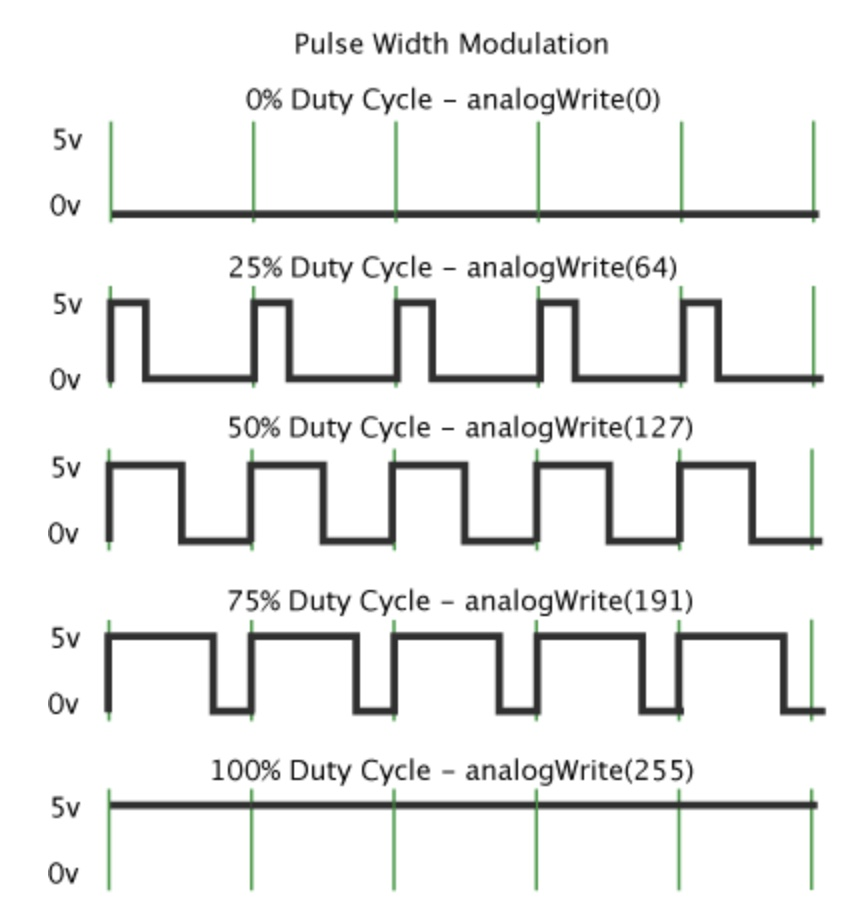
\includegraphics [width=13cm, height=8cm] {img/pulsweite} \newline \newline
Spezifischer ausgedrück passiert folgendes:
Eine Digitale Steuerung wird verwendet, um eine Rechteckwelle - ein Signal das zwischen Ein und Aus umgeschaltet wird
- zu erzeugen. Dieses Ein-Aus-Muster kann Spannungen zwischen der vollen Versorgungsspannung und Aus
simulieren.
Dabei wird der Anteil der Zeit geändert, den das Signal eingeschaltet ist im Vergleich zur Zeit, die das Signal
ausgeschaltet ist. Die Dauer der Einschaltzeit wird als Pulsweite bezeichnet. Um unterschiedliche analoge Werte zu
erhalten, wird die Pulsweite geändert bzw. moduliert. Wenn dieses Ein-Aus-Muster zum Beispiel schnell genug mit einer LED
wiederholt wird, resultiert daraus eine konstante Spannung zwischen 0 und Vcc, die die Helligkeit
der LED steuert. \newline
Auf den Arduino bezogen sieht die Umsetzung eines PWM Signals wie folgt aus:
Ein Taktsignal gelangt in die entsprechende Clock.
Die Clock stellt den entsprechenden PWM-Modus ein. Dabei werden zwei wichtige Werte gesetzt:
Der erste bestimmt, wann das Signal von HIGH auf LOW
umschaltet, während der zweite bestimmt, wann es zurückkommt. Das Verhältnis zwischen HIGH und LOW wird als
Tastverhältnis bezeichnet und bestimmt die Helligkeit unserer LED bzw. die Stärke, mit welcher der Hubmagnet anschlägt.
Je länger die Ausgabe im HIGH-Zustand bleibt, desto schneller erfolgt der Tastenanschlag. \newline
Neben dem Tastverhältnis, also das Verhältnis der Einschaltzeit zur
Periodendauer, welches oft in Prozent ausgedrückt wird, ist auch die Resolution (de: Auflösung) ein variierbarer Parameter.
Die Resolution bezieht sich auf die Anzahl der möglichen diskreten Werte, die das Signal annehmen kann.


\subsection{Vermehrung der Ausgänge}\label{output}
Da ein Klavier über 88 Tasten verfügt, müssen 88 Aktuatoren angesteuert werden. Ein Arduino hat keine 88 PWM-Ports, daher
müssen die Signale über eine Erweiterung der Ausgänge an die Motoren weitergegeben werden. Dafür gibt es mehrere Möglichkeiten:

\begin{enumerate}
	\item Schieberegister
	\item Motor-Matrix
	\item Demultiplexer
\end{enumerate}

\paragraph{Schieberegister}
Ein Schieberegister ist ein integrierter Schaltkreis, der hier verwendet wird, um die Anzahl der verfügbaren Ausgänge des
Mikrocontrollers zu erweitern. \newline
Um 88 Ausgänge mit Hilfe von Schieberegistern von nur 3 PWM-Pins des Arduinos anzusteuern, werden insgesamt 11 8-Bit-Schieberegister
(Also Schieberegister mit 8 Ausgängen) benötigt.\newline

Zuerst werden die Datenleitungen (SERIAL IN) aller Schieberegister in Reihe geschaltet. Dies bedeutet, dass das
Ausgangssignal des ersten Schieberegisters mit dem Eingang (SERIAL IN) des nächsten verbunden wird, und so weiter, bis
zum letzten Schieberegister. \newline
Der Arduino sendet Daten seriell über die verbundenen PWM-Pin. Diese Daten werden über ein Schieberegister an
alle Schieberegister weitergegeben. Durch diesen Vorgang werden die Daten parallel über alle Schieberegister gesendet.
\newline
Die Ausgänge der Schieberegister (Q0 bis Q7) werden dann an die entsprechenden Aktuatoren angeschlossen.
Das Signal wird zu einer definierten Clock durch die Schieberegister durchgeschoben. So kann durch Steuerung der Daten,
die an die Schieberegister gesendet werden, kann der Arduino jeden einzelnen Ausgang manipulieren, um die Aktuatoren
entsprechend anzusteuern. \newline
Auf diese Weise kann der Arduino mit Hilfe von Schieberegistern eine größere Anzahl von Ausgängen kontrollieren, als er
direkt verfügbar hat.


\paragraph{Motor-Matrix}
Die Motor-Matrix ist einer LED-Matrix nachgeahmt. //TODO: Picture Matrix and use muster to explain it for magnets
In einer Matrix, werden zwei Reihen an Ports angeschlossen, nach folgendem Muster:
$$
\begin{pmatrix}
	(11) & (12) & (13) & (14) & (15) & (16) & (17) & (18) \\
	(21) & (22) & (23) & (24) & (25) & (26) & (27) & (28) \\
	(31) & (32) & (33) & (34) & (35) & (36) & (37) & (38) \\
	(41) & (42) & (43) & (44) & (45) & (46) & (47) & (48) \\
	(51) & (52) & (53) & (54) & (55) & (56) & (57) & (58) \\
	(61) & (62) & (63) & (64) & (65) & (66) & (67) & (68) \\
	(71) & (72) & (73) & (74) & (75) & (76) & (77) & (78) \\
	(81) & (82) & (83) & (84) & (85) & (86) & (87) & (88)
\end{pmatrix}
$$


Eine LED-Matrix besteht aus einer Anordnung von LEDs in Zeilen und Spalten. Jede LED kann unabhängig von den anderen
ein- oder ausgeschaltet werden. Die Steuerung erfolgt über Multiplexing, bei dem jede Zeile der Matrix nacheinander
aktiviert wird, während die entsprechenden LEDs in den Spalten gleichzeitig eingeschaltet werden. Durch schnelles
Wechseln zwischen den Zeilen (PWM) erscheint es den BetrachterInnen, als ob alle LEDs gleichzeitig leuchten würden,
obwohl sie tatsächlich nacheinander aktiviert werden. \newline

Um das Prinzip einer LED-Matrix auf Aktuatoren zu übertragen, müssen lediglich die LEDs durch die Aktuatoren ersetzt werden.
Durch Steuerung der Zeilen und Spalten dieses Rasters können verschiedene Motoren selektiv
aktiviert werden. Dies ermöglicht eine effiziente Steuerung mehrerer Motoren mit einem begrenzten Satz von
Steuersignalen. \newline

//TODO: Nachteile Matrix


\paragraph{Demultiplexer}
//TODO

\subsection{Transistor}
Durchlaufspannung, Mindestspannung
\subsection{Aktuator}\label{subsec:aktuator}

\subsection{Schaltplan}

\textit{Arduino}

Im Zentrum der Schaltung steht der Mikrocontroller (hier: Arduino Uno R3).
Dieser erhält Daten und Strom über den integrierten USB-Anschluss, welcher mit dem Computer verbunden wird.
Da der Arduino limitierte \nameref{PWM}-fähige Ausgänge bereitstellt, werde Schieberegister (74HC595) verwendet.
Mit jedem \"in Reihe" geschaltetem Schieberegister kann die Anzahl PWM-fähiger Ausgänge um 8 erweitert werden.

\textit{Schieberegister}

Der Arduino wird an fünf Stellen mit dem ersten Schieberegister verbunden:

Arduinoport D2 <-> Serial (SER) Input

Über diese Verbindung werden serielle Daten werden hier bitweise in das Register geschoben.

Arduinoport D3 <-> SHCP (Shift Register Clock Input)

Dieser Pin wird verwendet, um den Takt für das Verschieben der Daten innerhalb des Schieberegisters anzulegen.
Bei jedem Taktimpuls auf diesem Pin wird das Bit am seriellen Dateneingang in das Register verschoben.
Das bedeutet, dass bei jeder steigenden Flanke des Taktsignals das Datenbit, das am Eingang anliegt, in das Schieberegister übernommen und alle vorhandenen Daten um eine Position verschoben werden.

Arduinoport D4 <-> STCP (Storage Register Clock Input)

Nachdem die Daten in das Schieberegister eingelesen wurden, wird dieser Pin verwendet, um die im Schieberegister vorhandenen Daten in das Ausgangsregister zu übertragen.
Ein Taktimpuls auf diesem Pin bewirkt, dass die Daten vom Schieberegister ins Ausgangsregister übernommen werden, sodass alle Ausgänge gleichzeitig aktualisiert werden.
Das ist besonders relevant, da sonst unter Umständen alle Ausgänge von einer Änderung im letzten Schieberegister bedingst wären.

Arduino GND <-> Ground, Output Enable (OE)

Der OE-Pin wird genutzt, um die Ausgänge des Schieberegisters global zu aktivieren oder zu deaktivieren, ohne die Daten selbst zu beeinflussen.
Da das Schieberegister zu keiner Zeit deaktiviert sein soll, wird dieser Pin dauerhaft mit dem GND-Pin verbunden.

Arduino VCC 5V <-> VCC, $\overline{SRCLR}$ (Reset)

Um das Schiebregister mit den benötigten 5V zu betreiben, wird der entsprechende Pin mit dem 5V Output des Arduino verbunden.
Zusätzlich wird der $\overline{ }$ SRCLR Port des Schieberegisters, welcher ein Reset ermöglicht dauerhaft mit 5V verbunden.

Jedes weiteres Schieberegister greift die oben genannten Signale ab.
Der einzige Unterschied befindet sich am Serial (SER) Input Port.
Das Schieberegister an Position i+1 wird mit dem seriellen Output des Schieberegisters an Position i verbunden. ($\forall i = 0,...,10$)

\textit{MOSFET}

Die Hubmagnete werden jeweils mit 24V und mit bis zu 400mA betrieben.
Um einen hohen Stromfluss zu steuern, können Transistoren verwendet werden.
Für hohe Spannungen und schnelle Schaltvorgänge eigenen sich besonders MOSFETs (Metall-Oxid-Halbleiter-Feldeffekttransistor).
Im Folgenden werden speziell n-MOSFETs verwendet, der mit einem Signal zwischen 0V (leitet nicht) und +5V (voll leitend) angesteuert werden kann.

Der folgende Aufbau ist für die insgesamt 88 Ausgänge der 11 Schieberegister identisch, da jeder Ausgang für die Ansteuerung genau eines Motors zuständig ist.

Der GATE-Pin des MOSFETs erhält das Signal, dass die \"Durchlässigkeit" steuert aus einem der Outputs des Schieberegisters.
Der SOURCE-Pin wird mit Ground des gesamten Systems verbunden.
Der DRAIN-Pin wird direkt mit dem entsprechenden Kontakt am Hubmagneten verbunden.

\textit{Hubmagnet}

Um den Stromkreis zu schließen wird der andere Kontakt des Hubmagnetes mit dem +24V verbunden.

\textit{Testen}

Um die Fehlersuche zu erleichtern, werden LEDs in den Schaltplan mit eingebaut.
Diese werden jeweils mit einem entsprechenden $1k\Omega$ Widerstand parallel zu den Motoren angeschlossen.
So kann anhand der Helligkeit der LED die Intensität abgelesen werden, mit der eine Taste gespielt wird.

//Bild vom Schaltplan

\section{Mechanik}\label{vorgehenHW}

\subsection{Auswahl des Klaviers}

Da sich dieses Projekt nicht auf die theoretische Konzeption beschränkt, muss ein entsprechendes Testobjekt - ein reales Klavier - gefunden werden.
Dieses muss einige Voraussetzungen erfüllen:
\begin{enumerate}
	\item 	Der Preis muss im Rahmen des Budgets (gesamt < 2000 €) liegen
	\item 	Es muss leicht auseinander zu bauen sein, um die Mechanik zugänglich zu machen
	\item 	Es muss vollständig sein (alle 88 Tasten)
	\item 	Es muss stimmbar sein
	\item 	Der Transport muss einfach durchzuführen sein
\end{enumerate}


\subsection{Ansteuerungskonzept}

//Drücken der ziehen, oben oder unten...
1. Oben
	Klavierhand
	Schiene
	Aufsatz mit 88 oben drüber
2. unten
	ziehen
	drücken

\subsection{Anbringung der Aktuatoren}
Beim Ansteuerungskonzept der Tasten muss auch beachtet werden, wo die Magnete befestigt werden.
Wir haben ein Brett, auf welchem sie befestigt werden. Folgende Bedenken:
1. Wie viel Platzt zwischen Solenoids?-weil Hitze
bsp. weiß unten und schwarz oben, weil die weißen weiter vorne
	-> nicht weil funktionalität vor optik (weil zu eng)
 -> Platz maximieren

2. Wie verbinden ohne dass Angelschnuren und andere Solenoids sich in den weg kommen
(3. spezifischer . in 2 oder 3 Reihen)
Voteil: Hitze
Nachteil: Umlenkung, Verkabelung

4. Umlenkung, damit der ganze Hub verwendet werden kann

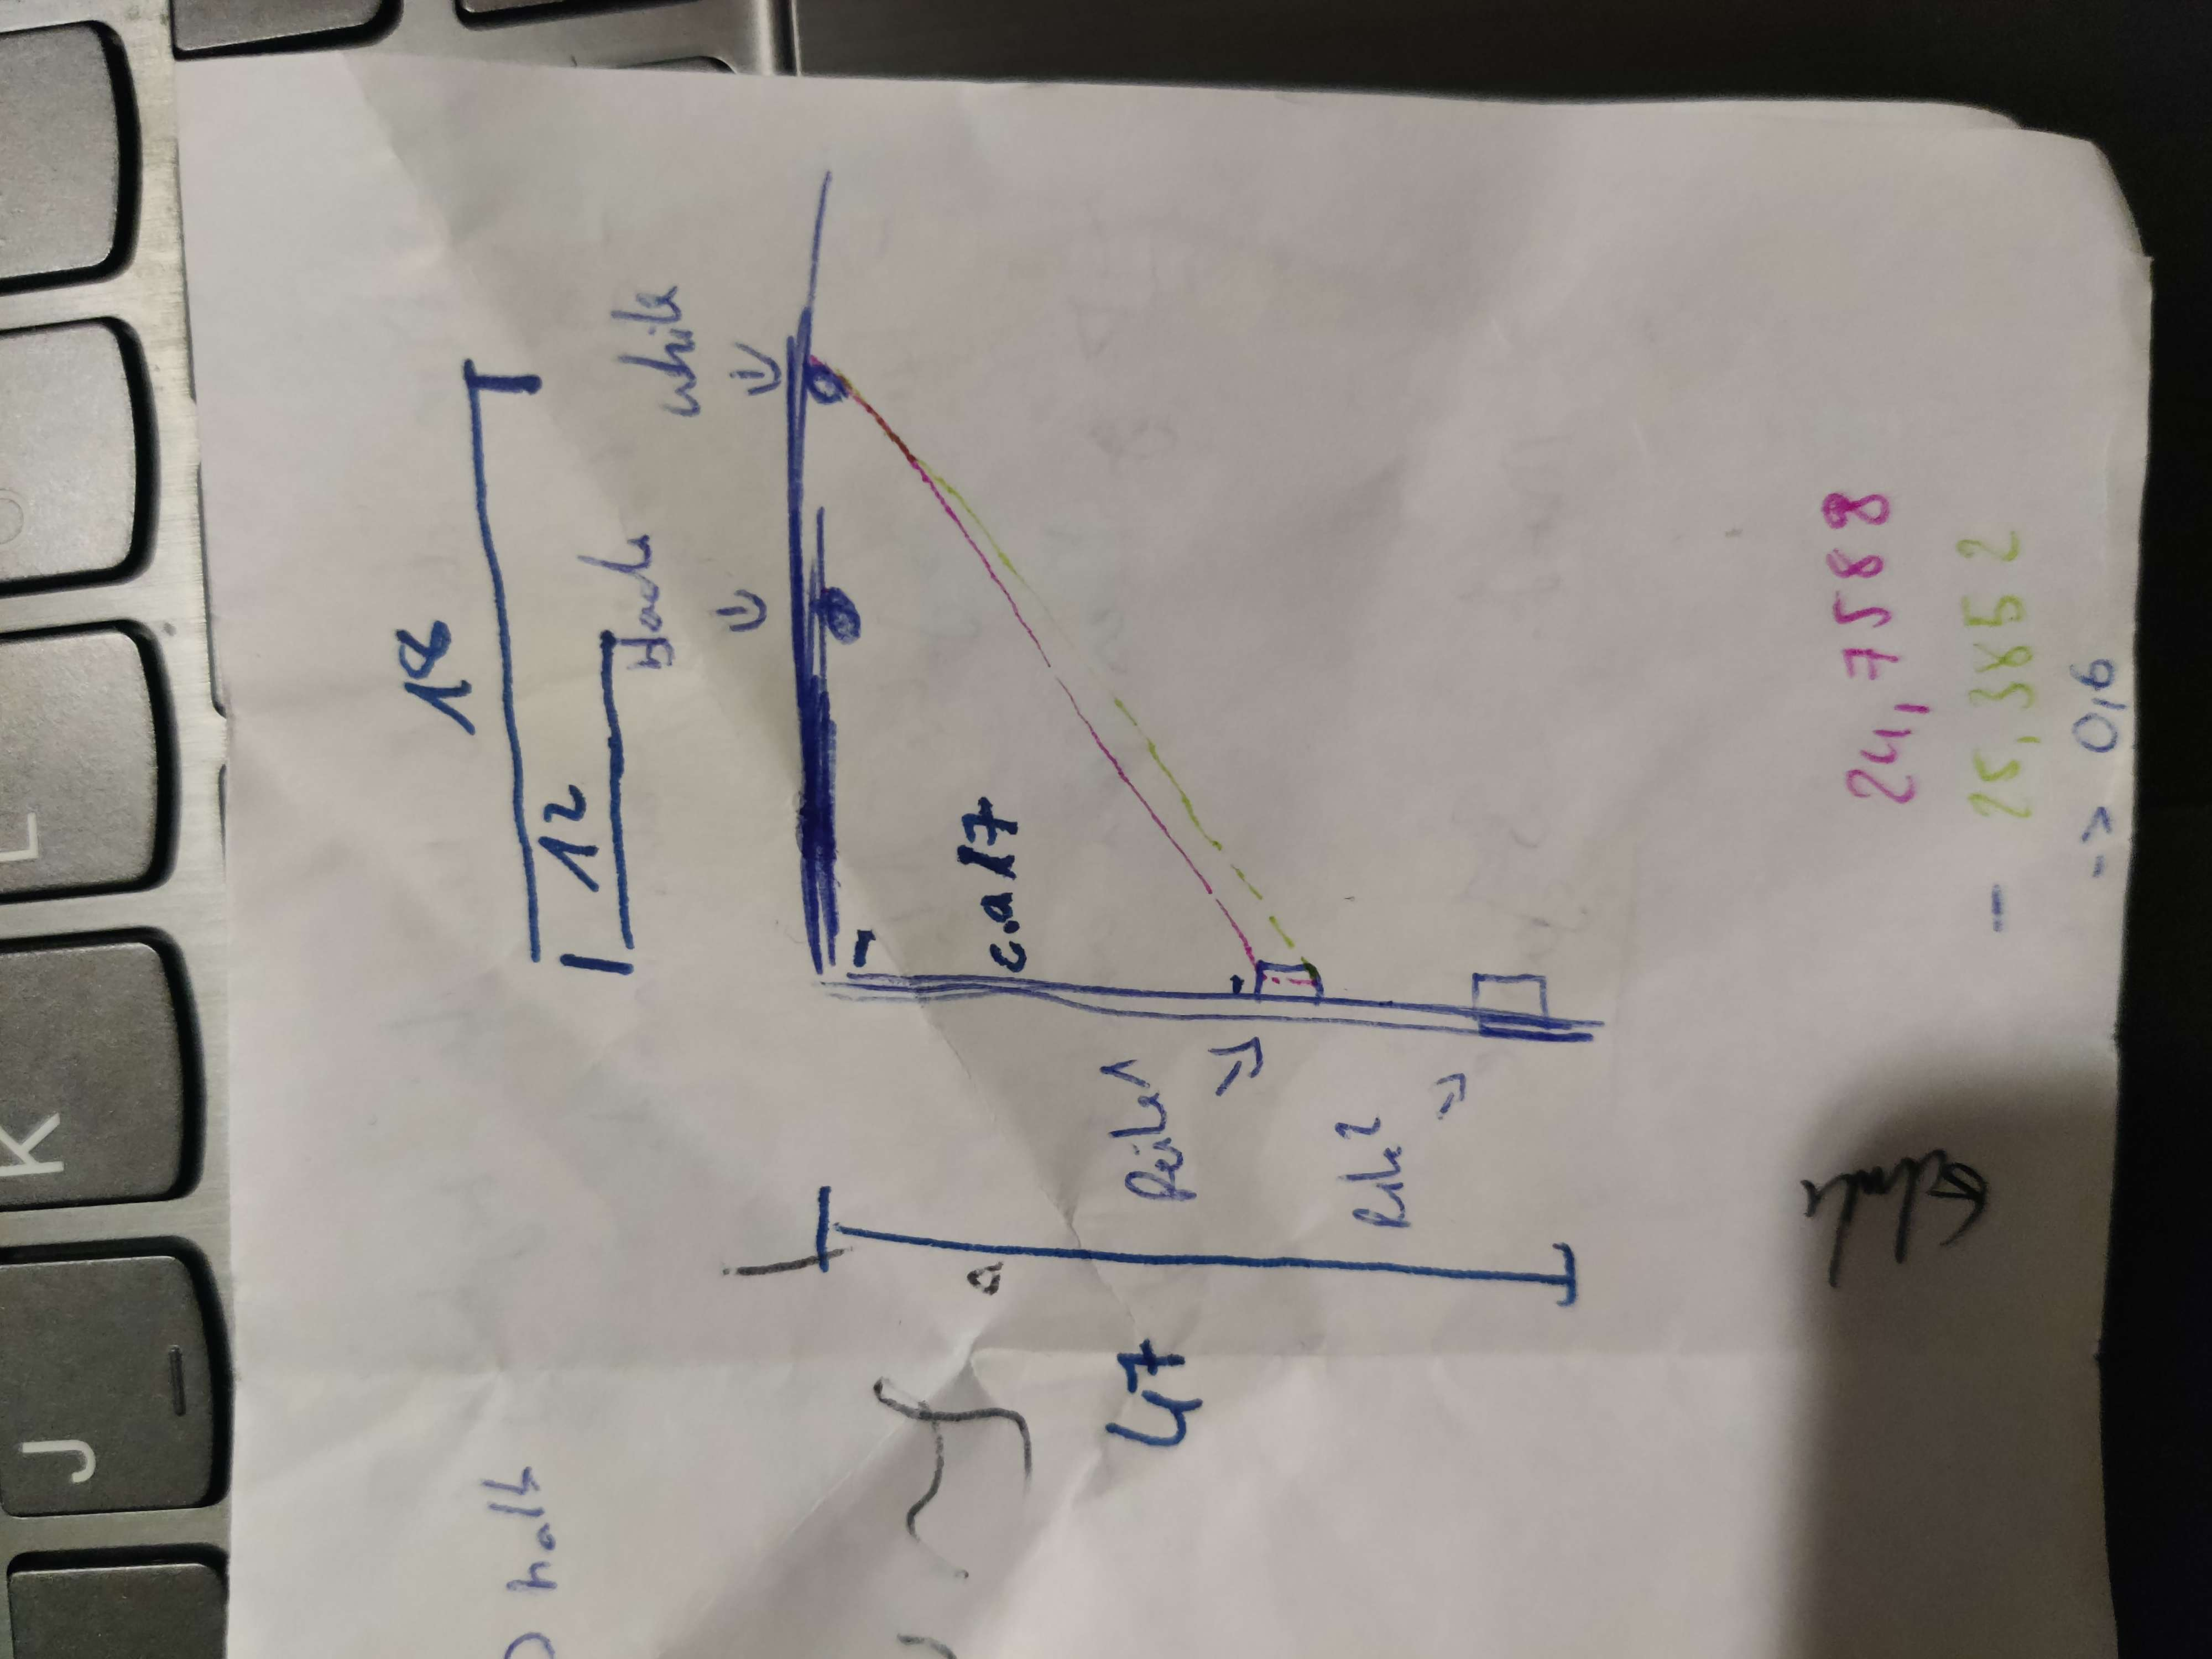
\includegraphics [width=5cm, height=4cm,angle=-90] {img/skizze_Umlenkung}

*Bild wegen Umlenkung

Erklärung geben: Haben Brett mit 67x25cm für 44 Motoren
*Bild von Brett-Sikzze



\subsection{Verbindung Tasten und Hubmagnete}

Es wurde sich dazu entschieden die Tasten durch Ziehen anzusprechen (siehe:\nameref{Ansteuerung}).
Die Grundidee ist, eine Schnur, oder Ähnliches, durch ein waagerechtes Loch in der Taste zu befestigen.
Anschließend wird die Schnur durch ein senkrechtes Loch durch das Holz, worauf die Tasten liegen, in den Fußraum geführt.
Damit der Pianist:in nicht durch Platzmangel eingeschränkt wird, werden die Seile entlang der Verkleidung zum Rumpf des Klaviers geführt.
Dort werden die Hubmagnete über die gesamte Breite befestigt.
Um die Intensität des Tastendrucks zu steuern und die Durabilität des Materials zu verlängern, sollte die Reibung möglichst gering gehalten werden.
Dazu wird mittels eines Rohres, welchen waagerecht unter der Klaviatur entlang der Löcher montiert wird als erste Umlenkung verwendet.


Für das Ziehen wird ein leichtes, formbares und dünnes Material benötigt, da Konzept die eine Seite mit dem Motor und die andere durch ein Loch in der Taste verknotet werden sollte.

\textit{Nähgarn}

Als Erstes wurden Nähgarn, welches zur Hand war getestet.
Auch doppelt hielt es der ruckartigen Ziehbewegung mit 25N des Hubmagnetens nicht stand.
Vier Fäden funktionierten zu Beginn gut, leierten allerding schnell aus.

\textit{Nylonsaiten}

Als Nächstes wurde die g-Saite einer Gitarre verwendet.
Durch den höheren Durchmesser und das stärkere Material riss und leierte die Saite nicht aus.
Da die Saite kaum Flexibilität liefert, war die Befestigung an der Taste äußerst schwierig.
Dadurch konnte nicht der vollständige Hub des Magnetes auf die Taste übertragen werden.

\textit{Angelschnur}

Aus Erfahrungen aus dem Angelbereich konnte schnell eine geeignete Schnur gefunden werden.
Genauer handelt es sich um eine geflochtene Schnur aus Polyethylene.
Mit einem Durchmesser von 1.6mm ist sie nicht nur sehr dünn und flexibel, sondern kann auch bis zu 7kg standhalten.
Damit sollte das Spielen des Forellenquintetts von Schubert ein leichtes sein.



\subsection{Weitere Ideen und Limitationen}

Im Laufe der Konzeption traten mehrere Herausforderungen auf, welche aus Zeit- und Konsten- Gründen nicht weiter
behandelt wurden.
\paragraph{Anzahl der Aktuatoren}
Wie bereits erklärt, wurden insgesamt 88 Aktuatoren verbaut, womit jede Taste angespielt werden kann. Trotz der Anzahl an
Hubmagneten, werden maximal 10 Tasten glechzeitig angespielt. Dies liegt an der Stromversorgung. Ein Hubmagnet benötigt
eine Stromversorgung von etwa 0.4 Ampere, für 10 Aktuatoren sind das also 4 Ampere. Das Netzteil welches wir verwenden, ist auf
6(?) Ampere ausgelegt, wobei wir mit einem Netzteil getestet haben, welches 2,8 Ampere unterstützt. Es gibt Netzteile die
einen höheren Stromföuss ermöglichen, allerdings sind diese um weiten teurer als das Netzteil, für welches wir uns entschieden haben.
Es wäre auch möglich, ein zweites Netzteil parallel zu Schalten, wodurch die Kosten nicht dramatisch gestiegen wären.
Wir haben hier allerdings keinen Mehrwert mehr gesehen. Die Logik und Ansteuerung des Klaviers bleibt die gleiche, weswegen
wir bei einem Netzteil mit einem maximalen Stromfluss von 6 Ampere (und 24V Leistung) verblieben sind.

\paragraph{Pedalansteuerung}
Ein Klavier hat normalerweise zwei oder drei Pedale, welchedie dynamik und den Klang des Klaviers beeinflussen.
Diese sind schwerer anzuspielen als die Tasten und benötigen somit Leistungsfähigere Aktuatoren als wir für die
Tasten nutzen. Es gab eine Überlegung diese Aktuatoren zu besorgen, da die Pedale klangtechnisch Mehrwert bringen.
Außerdem hätten wir uns noch Gedanken bezüglich der Schaltug und des Signals machen können. Einerseits hätte ein weiteres
Schieberegister genutzt werden können, wobei das Signal angepasst wird das die letzten 6 Ausgänge nie ein Signal bekommen.
ANdererseits hätten die Pedale mit weiteren PWM Ports des Arduinos verbunden werden können und die Signale unabhängig von den
Schieberegistern erhalten können. Im Prinzip wäre die Idee hier allerdings wieder die selbe wie beim Rest des Projektes gewesen,
weswegen wir Kosten an den Aktuatoren und der extra Stromversorgung für die Pedale gespart haben und diese nicht ansteuern.

\paragraph{Klangdämpfung der Aktuatoren}
Die Hubmagnete machen beim Anschlagen Geräusche, welche von der Melodie des Klaviers ablenken. Es gab eine Überlegung,
diese zu Dämpfen undem das Innere der Hubmagnete mit Isolierfolie abgedeckt wird und die Geräusche somit nicht so
offensichtlich sind. Letztendlich war uns die Gefahr, dass die Hubmagnete durch die Isolierung überhitzen oder nicht ganz
zurück schellen zu hoch, als dass wir die Klangdämpfung umsetzen würden.

Notiz von Oli: siehe diy piano Anschlag dempfen, indem man mit gummi die Taste limitiert
Notiz von Oli: Motorlager verwenden zwischen Platte und Klavier
Notiz von Oli:
Aktuatoren Geräuschreduzierung Tests:

Weg normal: 10mm

1. Schaumstoff:

*siehe bild
reduzierung des Weges, abfangen bevor es klopft
hässlich
sehr leise
Weg: 9mm (-1)

2. Seil (2mm Durchmesser) um den Anker

kann nicht rutschen, da kante
Nachteil: reibung
sehr leise
Weg: 8mm (-2)
%%%%%%%%%%%%%%%%%%%%%%%%%%%%%%%%%%%%%%%%%%%%%%%%%%%%%%%%%%
%   Autoren des Abschnitts:
%   Jakob Kautz
%   Olivier Stenzel
%%%%%%%%%%%%%%%%%%%%%%%%%%%%%%%%%%%%%%%%%%%%%%%%%%%%%%%%%%

% !TEX root =  master.tex
\chapter{Umsetzung - Hardware} \label{umsetzungHW}
\chapterauthor{Jakob Kautz, Olivier Stenzel}

\nocite{*}
- Probleme, Schwierigkeiten, Änderungen während der Umsetzung

Nachdem die Planungsphase abgeschlossen war, mussten die Überlegungen umgesetzt werden.
Im Rahmen dieser Arbeit wurde ein Prototyp gebaut, welcher 8 Tasten anspielen kann.
Zusätzlich wurde die Elektronik mit LEDs so erweitert, dass man das Drücken von 40 Tasten simulieren kann. % @Note(Val): Entweder hier oder an späterer Stelle erwähnen, dass es an sich trivial aber halt zeitaufwendig wäre, mehr Tasten anspielbar zu machen
% @Note(Val): Ich würde hier vielleicht noch gar nicht erwähnen, dass nur 8 Tasten anspielbar sind, weil die ganze Umsetzung ja mit dem Ziel 88 Tasten anspielbar zu machen lief. Kostenschätzung, etc. sind deshalb ja auch höher. Vielleicht ist es besser hier zu sagen, dass das Ziel war, den Prototypen mit möglichst vielen spielbaren Tasten zu gestalten, aber nur 8 bis dato erledigt wurden

\section{Materialien}
\chapterauthor{Jakob Kautz}
\subsection{Liste der Bauteile}
%TODO(Jay): Fix List
\begin{table}[htbp]
    \centering
    \begin{tabular}{|m{3.8cm}|m{1.7cm}|m{8cm}|}
        \hline
        \textbf{Bauteil} &  \textbf{Anzahl} & \textbf{Begründung}  \\
        \hline
        Hubmagnete & 88 & jede Taste braucht einen Hubmagneten um angespielt zu werden \\ % @Note(Val): Erwähnen, dass nur 8 der Hubmagnete benötigt wurden
        \hline
        Stromversorgung & 1 & Externe Stromversorgung für die Aktuatoren, da diese mehr als die 5V Vcc des Arduinos brauchen \\
        \hline
        Arduino & 1 & Kommunikation \\
        \hline
        Breadboard & 2 & Kleinstromschaltung \\
        \hline
        Schaltplatine & 5 & Großstromschaltung\\ % @Note(Jay): Heißt das so?
        \hline
        Schieberegister & 11 & Weitergabe Signal\\
        \hline
        Kabel (10cm) & 352stck (bzw. $9\cdot40$ in Packs) & Verbindungen in der Schaltung mit Schätzung 4 Kabel pro Hubmagnet\\
        \hline
        Kabel (20cm) & 176stck (bzw.$5\cdot40$ in Packs) & Verbindungen zu den Hubmagneten \\
        \hline
        LEDs & 88 & Tests \\
        \hline
        1kOhm Widerstände & 90 & Sicherheit and shit \\
        \hline
        MOSFET & 90 & Steuerung Strom \\
        \hline
        Feste Anschlussblöcke & 88 & Anschluss von Schaltplatine zu Hubmagnet\\
        \hline
        Angelschnur (...cm) & 88 & Verbindung Hubmagnet und Taste \\
        \hline
    \end{tabular}
    \caption{Ergebnisse der Anforderungen}
    \label{table:Bauteile}
\end{table}

\subsection{Kostenübernahme}
Die vorher spezifizierte Hardware für den Schaltplan musste für die Erstellung des Prototypen offensichtlich besorgt werden.
Aufgrund der relativ hohen Kosten für eine Studienarbeit, wurde bei einer der betreuenden Firmen angefragt, ob diese die Kosten für das Projekt übernehmen würde.
Damit dies möglich war, wurde ein Kostenvoranschlag gestellt, in welchem die benötigten Materialien mit den geschätzten Kosten aufgeführt wurden. % @TODO(Val): Kostenanschlag wird wahrscheinlich eine Tabelle, also referenzier die einfach "(siehe Tabelle \ref{...})" oder so

% @TODO(Jay): Add Kostenschätzung

Der Kostenanschlag erwies sich im Laufe des Projektes als (teils) unrealistisch. Dies lag insbesondere an der Anforderung
der Firma. Die Schätzung der Kosten basierte auf Anbietern, bei welchen die Materialien möglichst günstig zu kaufen sind.
Durch Firmenreglungen mussten diese allerdings alle bei Conrad oder Reichelt
% @Note(Jay): Stimmt das so?
gekauft werden. Diese Anbieter verkaufen die Materialien für sehr viel mehr Geld. Die tatsächlichen Kosten liefen
letztendlich also auf folgende Beträge hinaus: \newline % @TODO(Val): Hier am besten auch einfach wieder nur die Tabelle referenzieren, statt sie unbedingt in die nächste Zeile zu quetschen
% @TODO(Jay): Tatsächliche Kosten

Der Kostenunterschied betrug daher insgesamt .
% @TODO(Jay): Add difference
Hierbei ist allerdings zu erwähnen, dass die Kostenschätzung passend gewesen wäre, wenn die Anbieter frei wählbar wären.

\section{Prototypenbau}
Ursprünglich sollte der Aufbau des in Kapitel \ref{subsec:schaltplan} spezifizierten Schaltplans via Steckbrettern und
Jumperkabeln umgesetzt werden.
Zu Beginn wurde dies auch so umgesetzt. Das Problem welches dadurch entstand, war, dass die gewählten Platinen den
benötigten Stromfluss nicht aushalten.\newline
Jeder Aktuator - also jede gedrückte Taste - zieht einen Strom von 0.7A. Um das Projekt möglichst sinnvoll umzusetzen,
sollte der Aufbau mindestens 10 Tasten gleichzeitig drücken können, was bedeutet, dass der Aufbau mindestens 7.0A
Stromfluss problemlos ausstehen muss.
% @TODO(Jay): Wie viel halten Platinen aus? Warum konnten wir ein paar Jumper-Kabel nutzen? Wann brauchten wir die dickeren? Tabelle für welche Kabeldicke für welchen Stromfluss
% @Note(Val): Wann haben wir entschieden, dass min. 10 Tasten gleichzeitig spielbar sein sollen? Wenn wir das als Anforderung haben wollen, muss das im Anforderungs-Kapitel auch erwähnt werden

Aus diesem Grund wurde die gesamte Schaltung, die nach dem Schieberegister kommt, auf einer Lochrasterplatine fest gelötet.
Hierfür wurde ein 3mm starker Draht für die Stromversorgung verwendet.

\subsection{Klavieranbau}
Im Rahmen des Protoypen wurde die Elektrik nicht fest am Klavier verschraubt.
Das Brett mit den Hubmagneten wurde stattdessen nur an das Klavier angelehnt, während die Angelschnüre die Verbindung zu den Tasten herstellen.
Gespannt werden die Seile durch eine Schrauben-Mutter Konstruktion (siehe Abschnitt \ref{subsec:VerbindungTastenAktuatoren}).

\subsection{Ergebnisse des Prototypen}
% @TODO(Val):
Das Anspielen klappt iwie aber noch hakelig.



%%%%%%%%%%%%%%%%%%%%%%%%%%%%%%%%%%%%%%%%%%%%%%%%%%%%%%%%%%
%   Autoren des Abschnitts:
%   Jakob Kautz
%   Olivier Stenzel
%%%%%%%%%%%%%%%%%%%%%%%%%%%%%%%%%%%%%%%%%%%%%%%%%%%%%%%%%%

% !TEX root =  master.tex
\chapter{Ergebnisse - Hardware} \label{ergebnisse}

\nocite{*}
- Was wurde umgesetzt
- Messungen der Umsetzungen
- Limitationen der Umsetzung

% !TEX root =  master.tex
\nocite{*}
\chapter{Vorgehen - Software} \label{vorgehenSW}

Wie in Kapitel \ref{Zielstellung} beschrieben, benötigt dieses Projekt einen Desktop-Anwendung für die Nutzer:innen-Interaktion mit dem selbst-spielenden Klavier.
Außerdem wurde in Kapitel \ref{Hardware - Konzeption} bereits aufgezeigt, dass für die Ansteurung der Motoren ein \ac{MC} verwendet werden soll, der natürlich auch eine bestimmte Software ausführen muss.
Beide Komponenten, das \ac{UI} und der \ac{MC}, sollen in diesem Kapitel konzipiert werden.

Abbildung \ref*{fig:high-level-komponenten} zeigt diese unterschiedlichen Komponenten, sowie den Datenfluss zwischen diesen.
Nutzer:innen werden in der Abbildung auch dargestellt, um eindeutig zu machen, dass Nutzer-Eingaben nur an die \ac{UI} gehen.
Der \ac{MC} erhält Daten zum abzuspielenden Musikstück von der \ac{UI} und schickt darauf basierend in regelmäßigen Intervallen \ac{PWM}-Signale an die Hardware.

\begin{figure}[htbp]
	\centering
	\begin{tikzpicture}[node distance=2cm, line width=0.25mm]
		% Code for drawing a stick figure as taken from https://tex.stackexchange.com/a/441952
		% \begin{tikzpicture}
		% 	\thicklines
		% 	\put(5,18){\circle{5}}
		% 	\put(5,7){\line(0,1){8}}
		% 	\put(5,7){\line(1,-2){5}}
		% 	\put(5,7){\line(-1,-2){5}}
		% 	\put(1,12){\line(1,0){8}}
		% \end{tikzpicture}
		\node (user) [rect] {User}; % @TODO: draw Useer as stick figure
		\node (ui) [rect, below of=user] {UI};
		\node (mc) [rect, right of=ui, xshift=1.5cm] {\ac{MC}};
		\node (hw) [rect, right of=mc, xshift=1.5cm] {Hardware};

		\draw [arrow] (user) -- (ui);
		\draw [arrow] (ui) -- (mc);
		\draw [arrow] (mc) -- (hw);
	\end{tikzpicture}
	\caption{Komponenten-Diagramm mit Datenfluss}
	\label{fig:high-level-komponenten}
\end{figure}

Da die Hardware-Komponente in vorherigen Kapiteln bereits behandelt wurde, soll hier nur die Architektur der \ac{UI} (in Abschnitt \ref{vorgehenSW-UI}) und des \ac{MC} (in Abschnitt \ref{vorgehenSW-MC}) erarbeitet werden.
Dabei soll die Kommunikation zwischen diesen beiden Komponenten in Abschnitt \ref{vorgehenSW-SPPP} ebenfalls seperat betrachtet und spezifiziert werden.
Damit können die beiden Komponenten relativ aufwandsarm verändert oder ausgetauscht werden, solange sie sich weiterhin an das selbe Kommunikations-Protokoll halten.

Weiterhin soll auch das Format, in dem Musikstücke auf dem \ac{MC} gespeichert werden, in Abschnitt \ref{vorgehenSW-PIDI} seperat entworfen werden.
Da der \ac{MC} eine möglichst hohe Geschwindigkeit für die Ansteuerung der Motoren erbringen soll, muss das Format eine performante Nutzung ermöglichen.
Auch muss das Format möglichst wenig Speicherplatz aufbrauchen, damit möglichst viele Daten auf einmal auf dem \ac{MC} gespeichert werden können.
Je mehr Speicherplatz das Format nämlich benötigt, desto öfter muss die \ac{UI} Daten an den \ac{MC} schicken, was einen hohen Zeitaufwand mit sich bringen kann.

Zuletzt soll außerdem auch die Architektur der \ac{UI} in zwei Teile geteilt werden.
Die \ac{UI} hat an sich drei klar separierbare Aufgaben.
Zum einen muss die \ac{UI} natürlich Nutzer:innen-Eingaben verarbeiten und ein graphisches Interface rendern.
Zum anderen muss die \ac{UI} wie bereits erwähnt auch Daten an den \ac{MC} schicken.
Wie in Unterkapitel \ref{vorgehenSW-SPPP} aufgezeigt wird, muss die \ac{UI} auch Daten vom \ac{MC} empfangen können.
Die UI muss zusätzlich zum Rendering und der Kommunikation aber auch noch das Importieren von Musikstücken erlauben.
Wie in \ref{Zielstellung} spezifiziert, sollen Nutzer:innen Musikstücke in bestimmten Dateiformaten an die Anwendung geben können, um diese danach auf dem selbst-spielenden Klavier abspielen zu können.
Konzeptionelle Überlegungen dazu werden in \ref{vorgehenSW-MIDI} erläutert.


\section{PIDI} \label{vorgehenSW-PIDI}
\begin{enumerate}
	\item Existierendes vs. Custom Format
	\item Darstellung von Tönen (nicht an geg. Piano mit 88 Tasten gebunden)
	\item Speicher vs Performanz im Design des Formats (inkl. Alternativen)
\end{enumerate}

\section{Logik des Microcontrollers} \label{vorgehenSW-MC}
kurzer Überblick, vllt. mit SADT-Diagramm

\section{UI-Arduino Kommunikation} \label{vorgehenSW-SPPP}
\begin{enumerate}
	\item Wie wird Kommunikation mit Arduino i.d.R. gelöst
	\item Grundlagen der Kommunikation (Files, Polling, etc.)
	\item Prinzip der minimalen Arbeit → Custom Protocol → SPPP
	\item Asynchrone Umsetzung → Threading bei UI; Message-Buffer bei Arduino
\end{enumerate}

\section{UI} \label{vorgehenSW-UI}
\begin{enumerate}
	\item Grundlagen: Immediate vs. Retained Mode UI
	\item Cached Immediate Mode
	\item Generelle Diskussion bzgl. API-Design vllt
\end{enumerate}

\section{Parsing von MIDI} \label{vorgehenSW-MIDI}
\begin{enumerate}
	\item Überblick über Midi
	\item Vergleich MIDI vs PIDI
\end{enumerate}
(Kapitel vllt uninteressant?)
%%%%%%%%%%%%%%%%%%%%%%%%%%%%%%%%%%%%%%%%%%%%%%%%%%%%%%%%%%
%   Autoren des Abschnitts:
%   Val Richter
%%%%%%%%%%%%%%%%%%%%%%%%%%%%%%%%%%%%%%%%%%%%%%%%%%%%%%%%%%

% !TEX root =  master.tex
\chapter{Umsetzung - Software} \label{umsetzungSW}
\chapterauthor{Val Richter}

\nocite{*}
% - Probleme, Schwierigkeiten, Änderungen während der Umsetzung \newline
% - vllt. kurze Code-Schnippsel von besonders interessanten Teilen

Es steht nun ein Konzept für die benötigten Datenstrukturen und das erwünschte Verhalten der Software-Komponenten.
Dieses Verhalten kann nun jedoch auf unterschiedliche Arten entwickelt werden.
Ein möglicher Ansatz für die Entwicklung sieht zum Beispiel initial eine Klassifizierung aller logischen Objekte zur Laufzeit des gewünschten Programms vor.
Daraufhin kann dann analysiert werden, wie diese Objekte miteinander kommunizieren müssen und welche Daten diese haben und teilen müssen, um das erwünschte Verhalten der Software zu bekommen.
Im Folgenden soll diese Entwicklungs-Strategie als \enquote{Top-Down}-Ansatz bezeichnet werden.
Ein Top-Down-Ansatz klingt verlockend, da es scheint, als würde damit direkt die erwünschte Software geschrieben werden können.
Oftmals scheitert dieses Vorgehen jedoch in der Praxis. % @TODO(Val): Quelle & (belegte) Gründe warum es scheitert

Ein alternativer, \enquote{Bottom-Up}-Ansatz ist der von Casey Muratori als \enquote{Semantic Compression} \cite{mur.SemanticCompression.14} Getaufte.
Statt das Programm basierend auf logischen Objekten zu teilen, wird hier stattdessen eine Teilung in Schritte des gewünschten Verhaltens vorgenommen.
Weiterhin ist diese Teilung iterativ und geschieht während der Entwicklung, statt als seperate Aufgabe davor - wie es im davor beschriebenen Top-Down-Ansatz der Fall ist.
Sobald ein Teil des erwünschten Verhaltens konkret definiert wurde, kann dies in der einfachsten Art entwickelt werden.
Hierbei werden Gedanken der Wartbarkeit erstmal ignoriert.
Auch werden Abstraktionen in diesem Schritt noch nicht fortgeführt.
Stattdessen wird hier nur betrachtet, ob das erwünschte Teilverhalten funktional richtig implementiert wurden.

Bevor nun jedoch der nächste Teil der Anwendung implementiert wird, kommt die Semantische Kompression.
Auf lang oder kurz wird es vorkommen, dass zwei Teile des Codes die selbe oder eine ähnliche Folge von Operationen durchlaufen.
Diesem Ansatz nach wird nun der Code nach solchen semantischen Duplikaten durchsucht.
Solche Duplikate können dann extrahiert werden und in einzelnen Funktionen oder Datenstrukturen komprimiert werden.
Diese Komprimierung ist dabei nicht unbedingt eine syntaktische Komprimierung sondern eine semantische \cite[vgl. ]{mur.SemanticCompression.14}.

Beide Strategien zielen am Ende auf Code mit den gleichen Attributen ab.
Der Code soll gut lesbar, wartbar und erweiterbar sein.
Der erste Ansatz nimmt dabei an, dass die Teilung in logische Objekte das Verständnis der Codebasis erleichtert.
Der Bottom-Up Ansatz streitet diese Annahme im Generellen ab und behauptet stattdessen, dass semantisch komprimierter Code besser lesbar und verständlich ist, da es keine unnötigen Abstraktionen gibt und die existierenden Abstraktionen noch so nah an der konkreten Aufgabe sind wie nötig.
Ähnlich argumentieren beide Strategien, dass sie jeweils höhere Wartbarkeit und Erweiterbarkeit liefern.
Der fundamentale Gegensatz der beiden Ansätze kann jedoch - wie an dem einen Beispiel hoffentlich sichtbar wurde - in ihrer Haltung gegenüber Abstraktion finden.

Im Top-Down Ansatz wird Abstraktion generell positiv betrachtet.
Die Entwicklung beginnt mit einer abstrakten Klassifikation vermutlich benötigter Objekte und seperiert die Entwicklung entlang dieser Objekte.
Eine falsch gewählte Struktur oder Abstraktion dieser Objekte kann die Entwicklung entsprechend stark erschweren.
Der Bottom-Up Ansatz steht Abstraktion dagegen kritisch gegenüber.
Abstraktion ist hier immer noch erwünscht, aber nur wenn die Abstraktion die Reduzierung logischer Duplizierungen mit sich bringt und nur genau so weit abstrahiert ist wie nötig.
Unnötige Abstraktion oder Abstraktion, die auf einem höheren Level als nötig für das zu lösende Problem ist, ist hier negativ konnotiert.
Weiterhin wird hier nicht angenommen, dass zu Beginn der Entwicklung genug Wissen und Expertise besteht, um eine sinnvolle Architektur für den Code finden zu können.
Stattdessen ist die Semantische Kompression ein Verfahren zum explorativen Finden einer solchen sinnvollen Architektur.
In der Implementierung dieses Projekts wurde der Ansatz der Semantic Compression verwendet, da Erfahrungen mit besser und schlechter strukturierter Software dessen Thesen eher unterstützen.

Neben dem Entwicklungsansatz gibt es noch andere Entscheidungen, die die gesamte Entwicklung beeinflussen.
So ist auch die Wahl der Programmiersprache eine substantive und weitreichende Entscheidung.
Hier wurde sich entschieden, die gesamte Implementierung in der Programmiersprache C\footnote{Streng genommen ist hier der ISO-Standard C99 gemeint \cite*[siehe ][]{iso.c99}. Der Einfachheit halber wird in dieser Arbeit jedoch nur von \enquote{C} gesprochen.} zu erstellen.
Da der \ac{MC} vergleichsweise nur sehr begrenzten Speicherplatz zur Verfügung hat, ist die manuelle Speicherverwaltung von C hier sehr wünschenswert.

Aber auch für die Entwicklung der \ac{UI}, wo der verfügbare Speicherplatz praktisch nicht begrenzt ist, wurde sich entschieden C zu verwenden.
Der hauptsächliche Grund dafür ist die Transparenz der Sprache.
Während viele Nachfolger von C versuchen ihre Semantik abstrakt halten, um die eigentliche Implementierung davon loskoppeln zu können, ist jedes Sprachkonstrukt in C direkt auf die genaue Umsetzung auf dem Computer abzubilden.
Das kann nicht nur generell die Entwicklung erleichtern, sondern auch bei der Entwicklung von \ac{UI}s im besonderen Maße hilfreich sein, da die Performanz der Anwendung hier eine große Rolle für die Usability spielt.
Und eine transparente Sprache kann die Entwicklung performanter Anwendungen, da die Arbeit, die von der CPU für eine Aufgabe getan werden muss, leichter zu sehen ist.

Auch erleichtert die Verwendung von C die direkte Nutzung der Windows-API, da die Verwendung eines \ac{FFI}s ausbleibt.
Das hat sich vor allem bei der Entwicklung der Kommunikation (siehe Abschnitt \ref{umsetzungSW-Kommunikation}) als sinnvoll erwiesen.
Zuletzt ist auch noch amzumerken, dass ein substantiver Beweggrund für die Wahl von C in der hohen Erfahrung der Entwicklerin mit der Sprache lag. % @Note(Val): Sollte ich mich in der 3. Person so selbst benennen?

% @TODO(Val): Abschnitt(e) zur Verwendung von Libraries???
% Neben der Wahl der Programmiersprache wurde ebenfalls entschieden eine möglichst minimale Anzahl von Libraries zu verwenden.
% Libraries wollen meist in vielen unterschiedlichen Situationen nutzbar sein und haben entsprechend allgemeinere Annahmen als Code, der speziell für einen Anwendungsfall geschrieben wurde.
% Libraries verstecken außerdem oftmals die Arbeit, die für eine Aufgabe geleistet werden muss.
% Da, wie eingangs erwähnt, eine hohe Transparenz des Codes erwünscht ist, ist dies hier als Nachteil von Libraries gesehen, auch wenn eben jene Eigenschaft des Versteckens oft als Vorteil von Libraries genannt wird. % @TODO(Val): Quelle dafür einfügen
% Zuletzt bringen Libraries auch immer die Möglichkeit von Bugs oder unerwünschten Nebeneffekten.

% Libraries können außerdem sowohl die Verständlichkeit und Wartbarkeit des Codes erhöhen als auch verringern.
% Die Verwendung einer Library erfordert, dass die Entwickler:in die API sowie die Nebeneffekte der Library versteht.
% Gleichzeitig kann eine Library auch zusammenhängenden Code örtlich sortieren, verwendeten Operationen verständliche Namen geben und deren Komplexität verstecken, bis die Entwickler:in diese Komplexität betrachten muss bzw. will.

% @TODO(Val): Abschnitt zur Verwendung von Prototypen während Konzept-Phase???
% Während der Implementierung kam es zu keinen Änderungen zu dem in Kapitel \ref{vorgehenSW} vorgestellten Plans.
% Das liegt u.a. daran, dass Teile der Konzeption während der Entwicklung von Prototypen, erstellt wurden.
% So wurden beispielsweise die Möglichkeiten der Kommunikation zwischen \ac{UI} und \ac{MC} mithilfe von Prototypen gefunden.
% Basierend auf den Ergebnissen des Prototypen, wurden dann die Vor- und Nachteile unterschiedlicher Ansätze gefunden und die in Kapitel \ref{vorgehenSW} genannten Entscheidungen getroffen.

Folgend sollen besonders interessante Teile der Entwicklung noch genauer betrachtet werden.
Da die \ac{UI} den größten Teil der endgültigen Codebasis stellt, ist es interessant zu sehen, wie der oben erwähnte Bottom-Up Ansatz hier abgeschnitten hat.
Entsprechend wird in Abschnitt \ref{umsetzungSW-UI} auf die entstandene Architektur der \ac{UI} eingegangen.
Auch sollen Schwierigkeiten, die während der Programmierung aufgekommen sind, beschrieben werden.
Hier sind vor allem die Implementierung der Kommmunikation (siehe Abschnitt \ref{umsetzungSW-Kommunikation}) und des \ac{MC}s (siehe Abschnitt \ref{umsetzungSW-MC}) von Interesse.


\section{UI} \label{umsetzungSW-UI}
- Grundlagen: Immediate vs. Retained Mode UI \newline
- Cached Immediate Mode \newline
- Generelle Diskussion bzgl. API-Design vllt \newline
- Raylib API \newline
- Parallelisierung basierend auf unabhängigen Codepaths (siehe Blogpost dazu) \newline
- Thread-Kommunikation über geteilten read-only Speicher \& Mutexes wenn notwendig \newline


\section{Kommunikation} \label{umsetzungSW-Kommunikation}
- Lesen/Schreiben der Daten auf Arduino \newline
	- Ring-Buffer zum Lesen \newline
	- Greedy Reading/Parsing bei Music-Nachrichten \newline
- Lesen/Schreiben der Daten auf Windows \newline
	- Finden von COM-Ports (EnumPorts vs. Register, etc.) \newline
	- Lesen/Schreiben wie bei Dateien \newline
	- keine native Möglichkeit fürs Polling \newline
	- Synchrones Lesen einer gesamten Nachricht kann zu langem Blocken führen \newline
	- Asynchrones Lesn funktioniert nicht \newline
	- Lesen einzelner Bytes zum Befüllen eines buffers (symmetrisch zu MC) \newline
	- Lesen in Endlosschleife in eigenem Thread \newline
	- Schreiben in Chunks (Chunk-Größe über Ausprobieren herausgefunden) \newline
% @Note(Val): Documentaion of COM-Ports: https://learn.microsoft.com/en-us/windows-hardware/drivers/serports/configuration-of-com-ports


\section{Arduino-Programmierung} \label{umsetzungSW-MC}

- Arduino-Programmierung \newline
	- Bugs durch begrenzten Speicherplatz \newline
	- Berechnung von Oktave+Note zu Aktuator-Index \newline
	- Strategie für PlayedKeys Elimination \newline
- Code der zwischen UI und MC geteilt wurde \newline

% - Piano Layout (7 Oktaven, 3 Tasten davor, 1 Taste danach)\newline
% - Maximale Anzahl gleichzeitig laufender Motoren\newline
% - Werte durch Ausprobieren erraten (Minimaler Wert um Motor anzukriegen; Clock-Rate)\newline
% - Begrenzter Speicherplatz\newline
% - Konstante ‘Framerate’ ohne delay

% !TEX root =  master.tex
\chapter{Diskussion} \label{diskussion}

\nocite{*}
- Was wurde umgesetzt \newline
- UX & UI Design (kurz) \newline
- Limitationen der Umsetzung (nur MIDI, kein Image→/Ton→PIDI; etc.)
%%%%%%%%%%%%%%%%%%%%%%%%%%%%%%%%%%%%%%%%%%%%%%%%%%%%%%%%%%
%   Autoren des Abschnitts:
%   ???
%%%%%%%%%%%%%%%%%%%%%%%%%%%%%%%%%%%%%%%%%%%%%%%%%%%%%%%%%%

% !TEX root =  master.tex
\chapter{Zusammenfassung} \label{fazit}

\nocite{*}

- Abschließender Überblick über unsere Arbeit \newline
- Was lässt sich aus der Arbeit lernen? Was lief gut/schlecht? \newline
- Projekt in größeren Kontext setzen \newline
- Thema: Höhere Kosten als erwartet \newline
- Fazit ziehen

\section{Fazit}

...

\section{Ausblick}

...


%%%%%%%%%%%%%%%%%%%%%%%%%%%%%%%%%%%

%%%%%%%%%%%%%%%%%%%%%%%%%%%%%%%%%%%
% ANHÄNGE
%
% @stud: einzelne Anhänge bearbeiten und eigene Anhänge hier einfügen
%        die nachfolgenden Zeilen deaktivieren, wenn keine Anhänge verwendet werden
%
\initializeAppendix
% !TEX root =  master.tex
\chapter{Beispiel-Anhang: Testanhang}
Anh\"ange\index{Anhang} werden am Ende Ihrer Arbeit vor dem Literaturverzeichnis und dem Index eingef\"ugt.

\section{Abschnitt im Anhang}

Blabla

\section{Noch ein Abschnitt im Anhang}

\lipsum

% !TEX root =  master.tex
\chapter{Beispiel-Anhang: Noch ein Testanhang}
nochmal: lipsum ...

%%%%%%%%%%%%%%%%%%%%%%%%%%%%%%%%%%%

\singlespacing

%%%%%%%%%%%%%%%%%%%%%%%%%%%%%%%%%%%
% LITERATURVERZEICHNIS
% @stud: Literaturverzeichnis in Datei bibliography.bib anpassen.
%
% Alternative zu Verwendung von \initializeBibliography: Citavi ...
% (dann \initializeBibliography auskommentieren und eigenes LaTex Coding verwenden)
%
\initializeBibliography
%%%%%%%%%%%%%%%%%%%%%%%%%%%%%%%%%%%

%%%%%%%%%%%%%%%%%%%%%%%%%%%%%%%%%%%
% INDEX
% @stud: ggf. Index auskommentieren, wenn nicht benötigt
%
\addcontentsline{toc}{chapter}{Index}
\printindex

\end{document}
